As seen before, point clouds representations lack topological information.
An approach proposed by Wang et al.~\cite{Wang2019} involves constructing graphs associated with the point cloud, and then using a novel convolution operator, \textit{EdgeConv}.

\paragraph{EdgeConv} The edge convolution operates on a graph constructed from local regions of the point cloud.

Let $F$ be the feature number of each point in the point cloud. In the simplest case only the $(x,y,z)$ coordinates of the point are considered, so $F = 3$ but other features like RGB color can be used, for example if a 3D camera was employed to acquire the point cloud. In general $F$ is the dimensionality of the features in input to a layer.

To apply the edge convolution it must first be constructed a graph $G = (V,E)$, where $V \in \{1 \dots n\}$ are the vertices and $E \in V \times V$ are the edges. To construct a graph which represent a local structure in the point cloud a point is taken and then its $k$-nearest neighbors are computed. The graph will then have the points found as vertices and the connections between the point and its neighbors as edges.

An edge-feature is defined as $e_{ij} = h_{\Theta}(x_i, x_j) : R^F \times R^F \rightarrow R^{F'}$, where $h_{\Theta}$ is a non-linear function with $\Theta$ learnable parameters. The \textit{EdgeConv} operator is then defined by using an aggregation function $\square$ over the edge features associated with all the edges at each point. The output of EdgeConv at the vertex $x_i$ is:

\begin{equation}
\mathbf{x}_{i}^{\prime}=\underset{j:(i, j) \in \mathcal{E}}{\square} h_{\Theta}\left(\mathbf{x}_{i}, \mathbf{x}_{j}\right)
\end{equation}

After each EdgeConv layer the number of points in the point cloud remains the same, the input feature dimension is $F$ and the output feature dimension is $F'$.

\begin{figure}[ht]
    \centering
    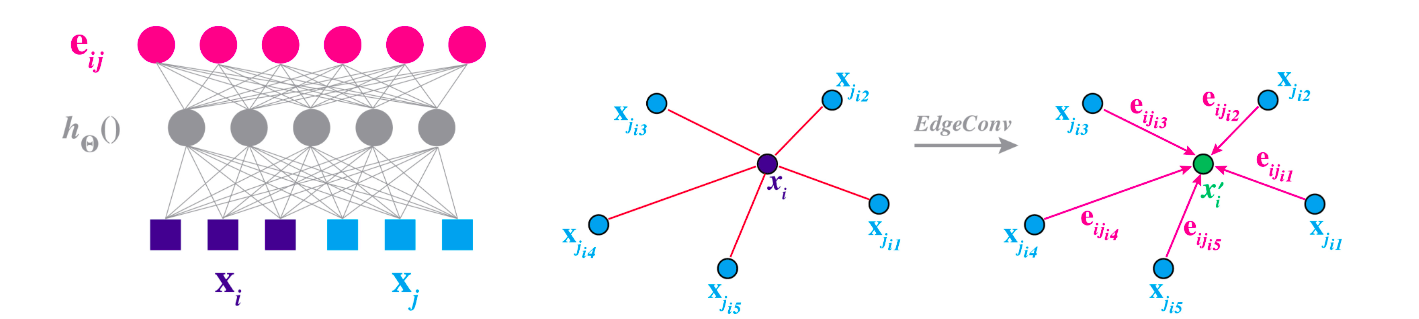
\includegraphics[width=\textwidth]{edgeconv.png}
    \caption{Left: the edge features $e_{ij}$, computed by a fully connected layer. Right: the edge features computed for each edge.~\cite{Wang2019}}
    \label{fig:edgeConvOperator}
\end{figure}

The choice of the $h_{\Theta}$ and $\square$ defines the properties of the EdgeConv operator. The authors of the paper chose an asymmetric edge function:

\begin{equation}\label{eq:edgeconv_h}
h_{\mathbf{\Theta}}\left(\mathbf{x}_{i}, \mathbf{x}_{j}\right)=\bar{h}_{\mathbf{\Theta}}\left(\mathbf{x}_{i}, \mathbf{x}_{j}-\mathbf{x}_{i}\right)
\end{equation}

This function takes into account both the global structure by using the coordinates of $x_i$ and the local structure by using the distances between $x_i$ and its neighbors. This function is easily implemented by an MLP.

As for the aggregation function $\square$ the authors chose the max function:

$$
x_{i}^{\prime}=\max _{j:(i, j) \in \mathcal{E}} e_{i j}^{\prime},
$$

The properties of the EdgeConv operator depend on the choice of the edge and aggregation functions.

Using the $\max$ aggregation achieves permutation invariance with respect to the order of the neighbor points $x_j$.

As for the translation invariance it can seen in equation~\ref{eq:edgeconv_h} that the operator is partially invariant on the translation. It is easy to demonstrate that $h_{\Theta}(x_i - x_j)$ is translation invariant, while $h_{\Theta}(x_i)$ isn't, as shown in equation~\ref{eq:edgeconv_tranls}.

\begin{equation}\label{eq:edgeconv_tranls}
\begin{split}
    \bar{h}_{\mathbf{\Theta}}\left((\mathbf{x}_{j} + T)-(\mathbf{x}_{i} + T), \mathbf{x}_{i} + T \right) = \\
    \theta \cdot ((\mathbf{x}_{j} + T)-(\mathbf{x}_{i} + T)) + \phi \cdot (\mathbf{x}_{i} + T) = \\
    \theta \cdot (\mathbf{x}_{j}-\mathbf{x}_{i}) + \phi \cdot (\mathbf{x}_{i} + T)
\end{split}
\end{equation}


If only the first part is considered then EdgeConv is fully invariant to translation, however the global structure information would be lost: the classification would be based on patches of the point cloud without taking into account the global pose of these patches.

\paragraph{Dynamic graph update}
An important part explored is the dynamic graph computation.
State of the art approaches in graph based network compute the graph at the beginning and then use it throughout the network. DGCNN instead recomputes the graph after each EdgeConv layer: the architecture learns how to construct the graph.
The k-nearest neighbors are found by computing the pairwise distance matrix in feature space.

\paragraph{Architecture and results}

The network architecture used for the evaluation experiments is shown in figure~\ref{fig:DGCNN}. It is composed of 4 EdgeConv layers with skip connections to aggregate multi scale features, obtaining a 512-dimesional point cloud, and a max pooling layer. Then there are multiple fully connected layers. All layers include leaky ReLU as activation function and batch normalization.

\begin{figure}[ht]
    \centering
    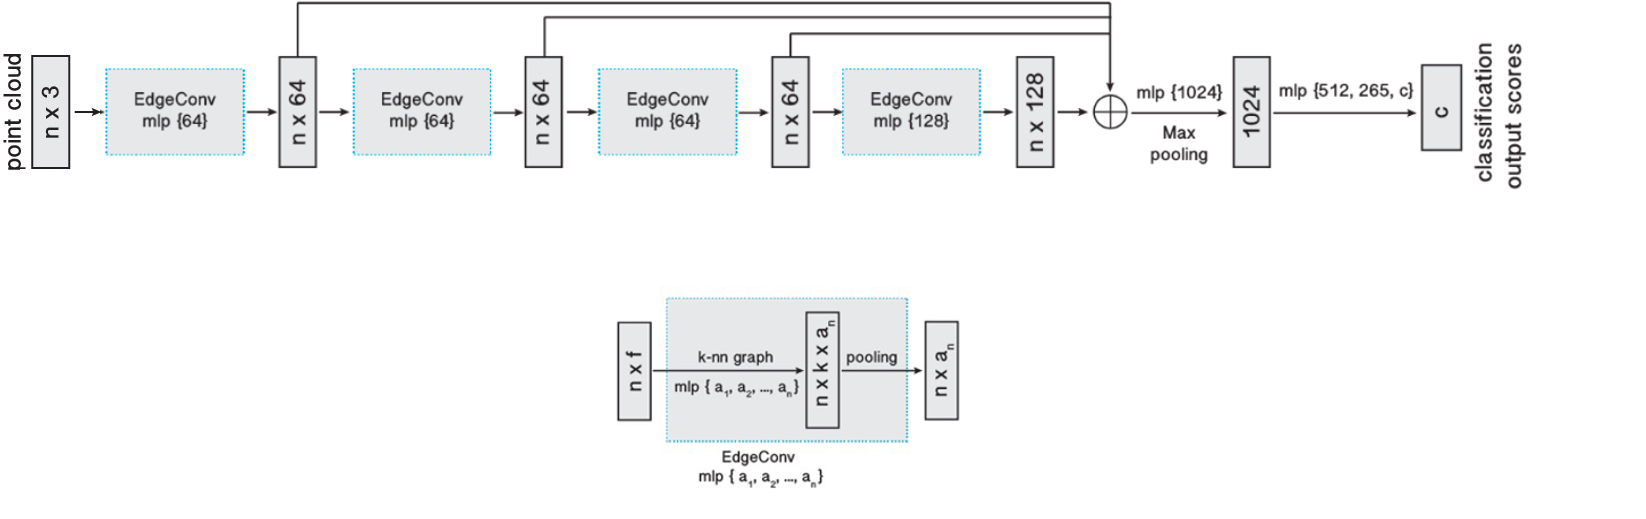
\includegraphics[width=\textwidth]{DGCNN_orig.png}
    \caption{Top: DGCNN network architecture. Bottom: EdgeConv.~\cite{Wang2019}}
    \label{fig:DGCNN}
\end{figure}

The experiments have been performed on ModelNet40, and have been conducted in the same way as PointNet authors did, which have become a standard to have a meaningful comparison between different networks.

The baseline model uses only a fixed graph (no dynamic computation), and uses as edge function $ h_{\Theta}(x_i, x_j)$. With this model an improvement of $\SI{1}{\percent}$ over PointNet++ is achieved.

Multiple experiments have been performed to evaluate how much each part of the model influences the accuracy results, as shown in table~\ref{tab:dgcnn_exp}.
Three improvements to the networks have been tried:

\begin{itemize}
    \item Centralization, which is using explicitly the global information given by the vertex $x_i$ and the distance between its neighbors, by using the edge function ${h}_{\mathbf{\Theta}}\left(\mathbf{x}_{i}, \mathbf{x}_{j}-\mathbf{x}_{i}\right)$.
    \item Dynamic graphs, which is the computation of the neighbors on the features extracted for each EdgeConv layer.
    \item More points, by using 2048 points instead of 1024.
\end{itemize}

\begin{table}[htb]
    \centering
    \caption{CENT denotes centralization, DYN denotes dynamical graph recomputation and MPOINTS denotes experiments with 2,048 points}
    \begin{tabular}{ccccc}
        \hline \text { CENT } & \text { DYN } & \text { MPOINTS } & \text { MEAN CLASS ACCURACY(\%) } & \text { OVERALL ACCURACY(\%) } \\
        \hline x & & & 88.9 & 91.7 \\
        x & x & & 89.3 & 92.2 \\
        x & x & x & 90.2 & 92.9 \\
        \hline
    \end{tabular}
    \label{tab:dgcnn_exp}
\end{table}

It is also worth noticing that DGCNN performs faster than state of the art network such as PointNet++, while keeping the model size relatively small, as shown in table~\ref{tab:dgcnn_exp2}.

\begin{table}[htb]
    \centering
    \caption{Size and time comparison between PointNet, PointNet++ and DGCNN }
    \begin{tabular}{lccc}
        \hline & \text { MODEL SIZE(MB) } & \text { TIME(MS) }  \\
        \hline \text { POINTNET (BASELINE) (QI ET AL. 2017B) } & 9.4 & 6.8  \\
        \text { POINTNET (QI ET AL. 2017B) } & 40 & 16.6 \\
        \text { POINTNET++ (QI ET AL. 2017C) } & 12 & 163.2 \\
        \text { DGCNN (BASELINE) } & 11 & 19.7  \\
        \text { DGCNN } & 21 & 27.2  \\
        \hline
    \end{tabular}
    \label{tab:dgcnn_exp2}
\end{table}